
%%%%%%%%%%%%%%%%%%%%%%%%%%%%%%%%%%%%%%%%%%%%%%%%%%%%%%%%%%
%%%%%%%%%%%%%%%%%%%%%%%%%%%%%%%%%%%%%%%%%%%%%%%%%%%%%%%%%%
\chapter{Quantitative Metrics for 2D Packings}
\label{chapter_qualitative_metrics}
%%%%%%%%%%%%%%%%%%%%%%%%%%%%%%%%%%%%%%%%%%%%%%%%%%%%%%%%%%
%%%%%%%%%%%%%%%%%%%%%%%%%%%%%%%%%%%%%%%%%%%%%%%%%%%%%%%%%%

\mynote
{
\begin{itemize}
\item adequacy, efficiency, productiveness, effectiveness (choose your criteria, state them clearly and justify them)
\item be careful that you are using a fair measure, and that you are actually measuring what you claim to be measuring
\item if comparing with previous techniques those techniques must be described in Chapter 2
\item be honest in evaluation
\item admit weaknesses
\end{itemize}
}

%%%%%%%%%%%%%%%%%%%%%%%%%%%%%%%%%%%%%%%%%%%%%%%%%%%%%%%%%%
%%%%%%%%%%%%%%%%%%%%%%%%%%%%%%%%%%%%%%%%%%%%%%%%%%%%%%%%%%
\section{Introduction}
%%%%%%%%%%%%%%%%%%%%%%%%%%%%%%%%%%%%%%%%%%%%%%%%%%%%%%%%%%
%%%%%%%%%%%%%%%%%%%%%%%%%%%%%%%%%%%%%%%%%%%%%%%%%%%%%%%%%%



\mynote{paragraph is so so...}

\newtext
{
As with many techniques in artistic applications of computer graphics, 
evaluating the quality of a computer-generated element packing is a challenge.
%We believe that results shown in this thesis meet the aesthetic goals
%we defined for this style of packing. 
We are particularly interested in investigating quantitative measurements of packing
quality that can be used to evaluate our results and subsequent
work. In this chapter, we compare 2D packings generated by RepulsionPak
with other packings created by other methods or artists.
}

\newtext
{
We believe that perceived packing quality is closely tied to the evenness
of negative space.
The separation between neighbouring elements should be roughly the same everywhere.
In the limit, as this element separation goes to zero,
the packing turns into a tessellation: a set of elements that exactly
fill a container with no overlaps. 
The challenge---and visual appeal---of packings
follows in part from aligning neighbouring elements along compatible 
segments of their boundaries, suggesting that they interlock by design.  
We have developed several measurements of evenness,
which allow us to examine the behaviour of manually constructed reference
packings and to compare RepulsionPak with other packing algorithms.
}


%%%%%%%%%%%%%%%%%%%%%%%%%%%%%%%%%%%%%%%%%%%%%%%%%%%%%%%%%%
%%%%%%%%%%%%%%%%%%%%%%%%%%%%%%%%%%%%%%%%%%%%%%%%%%%%%%%%%%
\section{Related Work}
%%%%%%%%%%%%%%%%%%%%%%%%%%%%%%%%%%%%%%%%%%%%%%%%%%%%%%%%%%
%%%%%%%%%%%%%%%%%%%%%%%%%%%%%%%%%%%%%%%%%%%%%%%%%%%%%%%%%%

\mynote{Find figures here C Users azer OneDrive meetings meeting old ones}

We build a distance transform by calculating the distance of every pixel in the negative space
to the nearest element boundary.


Voronoi Diagrams

Medial Axis

%%%%%%%%%%%%%%%%%%%%%%%%%%%%%%%%%%%%%%%%%%%%%%%%%%%%%%%%%%
%%%%%%%%%%%%%%%%%%%%%%%%%%%%%%%%%%%%%%%%%%%%%%%%%%%%%%%%%%
\section{Quantitative Metrics}
%%%%%%%%%%%%%%%%%%%%%%%%%%%%%%%%%%%%%%%%%%%%%%%%%%%%%%%%%%
%%%%%%%%%%%%%%%%%%%%%%%%%%%%%%%%%%%%%%%%%%%%%%%%%%%%%%%%%%

\newtext
{
Two packings must be calibrated to each other before our measurements 
can be compared meaningfully.  
We can compare packings of different sizes by normalizing their containers to
have unit area.  We must also arrange for the packings to have the same
} % newtext ends here
\textit{negative space ratio} 
 \newtext
{(the overall amount of negative space as a 
fraction of container area), so that our measurements can focus on the
distribution of negative space and not just the amount.  Given two
calibrated packings, we examine three main evenness metrics:
overlap of offset elements, spherical contact probability functions,
and distance histograms. %We discuss each of these metrics in detail below.
}

%%%%%%%%%%%%%%%%%%%%%%%%%%%%%%%%%%%%%%%%%%%%%%%%%%%%%%%%%%
%%%%%%%%%%%%%%%%%%%%%%%%%%%%%%%%%%%%%%%%%%%%%%%%%%%%%%%%%%
\subsection{The Overlap Function}
%%%%%%%%%%%%%%%%%%%%%%%%%%%%%%%%%%%%%%%%%%%%%%%%%%%%%%%%%%
%%%%%%%%%%%%%%%%%%%%%%%%%%%%%%%%%%%%%%%%%%%%%%%%%%%%%%%%%%

The overlap function is a function of a non-negative offset amount
$r$.  For any given $r$, we offset every element by computing its Minkowski
sum with a disc of radius $r$.  As $r$ grows, elements will start overlapping;
the overlap function measures the total area of these overlaps, normalized
by container area, as a function of $r$.  We can also visualize these 
overlapping areas directly as in Figure~\ref{fig_overlap_function}.  In a 
perfect packing, we would expect no overlaps until $r=d_\mathrm{gap}/2$,
our desired gap distance, at which point overlapping areas would start to
grow into channels of roughly even width.

%%%%%%%%%%%%%%%%%%%%%%%%%%%%%%%%%%%%%%%%%%%%%%%%%%%%%%%%%%
%%%%%%%%%%%%%%%%%%%%%%%%%%%%%%%%%%%%%%%%%%%%%%%%%%%%%%%%%%
\subsection{Spherical Contact Probability}
%%%%%%%%%%%%%%%%%%%%%%%%%%%%%%%%%%%%%%%%%%%%%%%%%%%%%%%%%%
%%%%%%%%%%%%%%%%%%%%%%%%%%%%%%%%%%%%%%%%%%%%%%%%%%%%%%%%%%

The spherical contact probability (SCP) is the probability that a 
disc of radius $r$, chosen
uniformly at random within the container region, lies entirely within the 
packing's negative space~\cite{Chiu2013}.
The SCP can be summarized via a function $Q_s(r)$ that gives this 
probability for each radius $r$.
In order to interpret the SCP, it is helpful first to
examine a ``packing'' with perfectly even negative space (Figure~\ref{hsr_viz}a).
Consider a pattern of infinite horizontal stripes of width $d_\mathrm{s}$,
separated from each other by $d_\mathrm{gap}$.  For this pattern,
$Q_s(0)=d_\mathrm{gap}/(d_\mathrm{gap}+d_\mathrm{s})$; it is also
clear that $Q_s(d_\mathrm{gap}/2)=0$, because no disc of diameter greater
than $d_\mathrm{gap}$ can fit in the negative space
(our $d_\mathrm{gap}$ is twice the radius of the ball).
Furthermore,
$Q_s(r)$ will decrease linearly between these two points, and remain
at zero thereafter; its graph will consist of a tilted line segment
connected to a horizontal ray.

No real-world packing exhibits this SCP.  Even in a perfect arrangement
of squares (Figure~\ref{hsr_viz}b), the intersections of horizontal and
vertical channels
produce pockets of negative space that can accommodate balls of
radius $d_\mathrm{gap}\sqrt{2}/2$.  These pockets tend to raise the SCP
slightly everywhere, and cause it to bend into a small tail that
approaches zero gradually.
For a given set of elements in a container, the best packings will
have \newtext{a steeply-decreasing} SCP that stays close to the idealized stripe function most
of the way down, has a low value at $r=d_\mathrm{gap}/2$,
and then bends towards horizontal near that value.
Note that there is always a largest disc that can fit in a packing's
negative space, and hence a largest $r$ for which $Q_s(r)>0$.  
In our graphs, we plot $Q_s(r)$ only until this point, allowing us
to compare the largest empty gaps of two packings.
In less effective packings (Figs.~\ref{hsr_viz}c,d), the negative space 
will be narrower in
some places and wider in others, recognizable as a shallower SCP
with a longer tail.

\newtext{We geometrically compute SCP} by offsetting the negative
space inward.  Let $N$ be the shape of the negative space (essentially
the container region with holes where elements are).  For a given radius
$r$, we compute $N(r)$, the Minkowski difference of $N$ with a disc of
radius $r$.  Then $Q_s(r)$ is simply the ratio of the area of $N(r)$ to
the area of the container.

%%%%%%%%%%%%%%%%%%%%%%%%%%%%%%%%%%%%%%%%%%%%%%%%%%%%%%%%%%
%%%%%%%%%%%%%%%%%%%%%%%%%%%%%%%%%%%%%%%%%%%%%%%%%%%%%%%%%%
\subsection{Histograms of the Distance Transform}
%%%%%%%%%%%%%%%%%%%%%%%%%%%%%%%%%%%%%%%%%%%%%%%%%%%%%%%%%%
%%%%%%%%%%%%%%%%%%%%%%%%%%%%%%%%%%%%%%%%%%%%%%%%%%%%%%%%%%
The distance transform of the negative space can also provide insights into
how negative space varies.  We could calculate a standard \textbf{histogram of the
distance transform}, but that would require quantizing distances into bins.
Instead, note that the SCP $Q_s(r)$ is precisely the normalized area of 
negative space for which the distance transform is at least $r$. 
 Looked at another way, if we offset each element by a
   radius $r$, then $1-Q_s(r)$ must be the normalized 
     area of the union of these offset elements.
% Looked at
% another way, we can offset each element by a radius $r$, in which case 
% $1-Q_s(r)$ must be the normalized area of the union of these offset elements.
This area can then be interpreted as 
a cumulative distribution function of distance.  From this observation
we can compute a continuous variant of the distance histogram as a 
probability density function via the derivative of the SCP: $H(r)=-Q_s'(r)$.

\newtext{
Given two calibrated packings, the areas under their distance histograms
are the same.  But a more even packing will have a shorter tail,
indicating a tighter upper bound on gap size, and it will have a larger
concentration of density around $d_\mathrm{gap}/2$.  In Figure~\ref{hsr_viz},
the histogram for the perfect stripe pattern is a step function that drops
to zero at $d_\mathrm{gap}/2$.  The ideal square packing has a histogram
that climbs gently until around $d_\mathrm{gap}/2$ before dropping
steeply.  The other two packings have shallower, smoother histograms.
Note also that high values of the distance histogram near $d_\mathrm{gap}/2$
correspond to a rapid negative change in the SCP, suggesting a more even
packing.
}


%%%%%%%%%%%%%%%%%%%%%%%%%%%%%%%%%%%%%%%%%%%%%%%%%%%%%%%%%%
%%%%%%%%%%%%%%%%%%%%%%%%%%%%%%%%%%%%%%%%%%%%%%%%%%%%%%%%%%
\section{Comparisons}
%%%%%%%%%%%%%%%%%%%%%%%%%%%%%%%%%%%%%%%%%%%%%%%%%%%%%%%%%%
%%%%%%%%%%%%%%%%%%%%%%%%%%%%%%%%%%%%%%%%%%%%%%%%%%%%%%%%%%


\begin{figure}
\centering
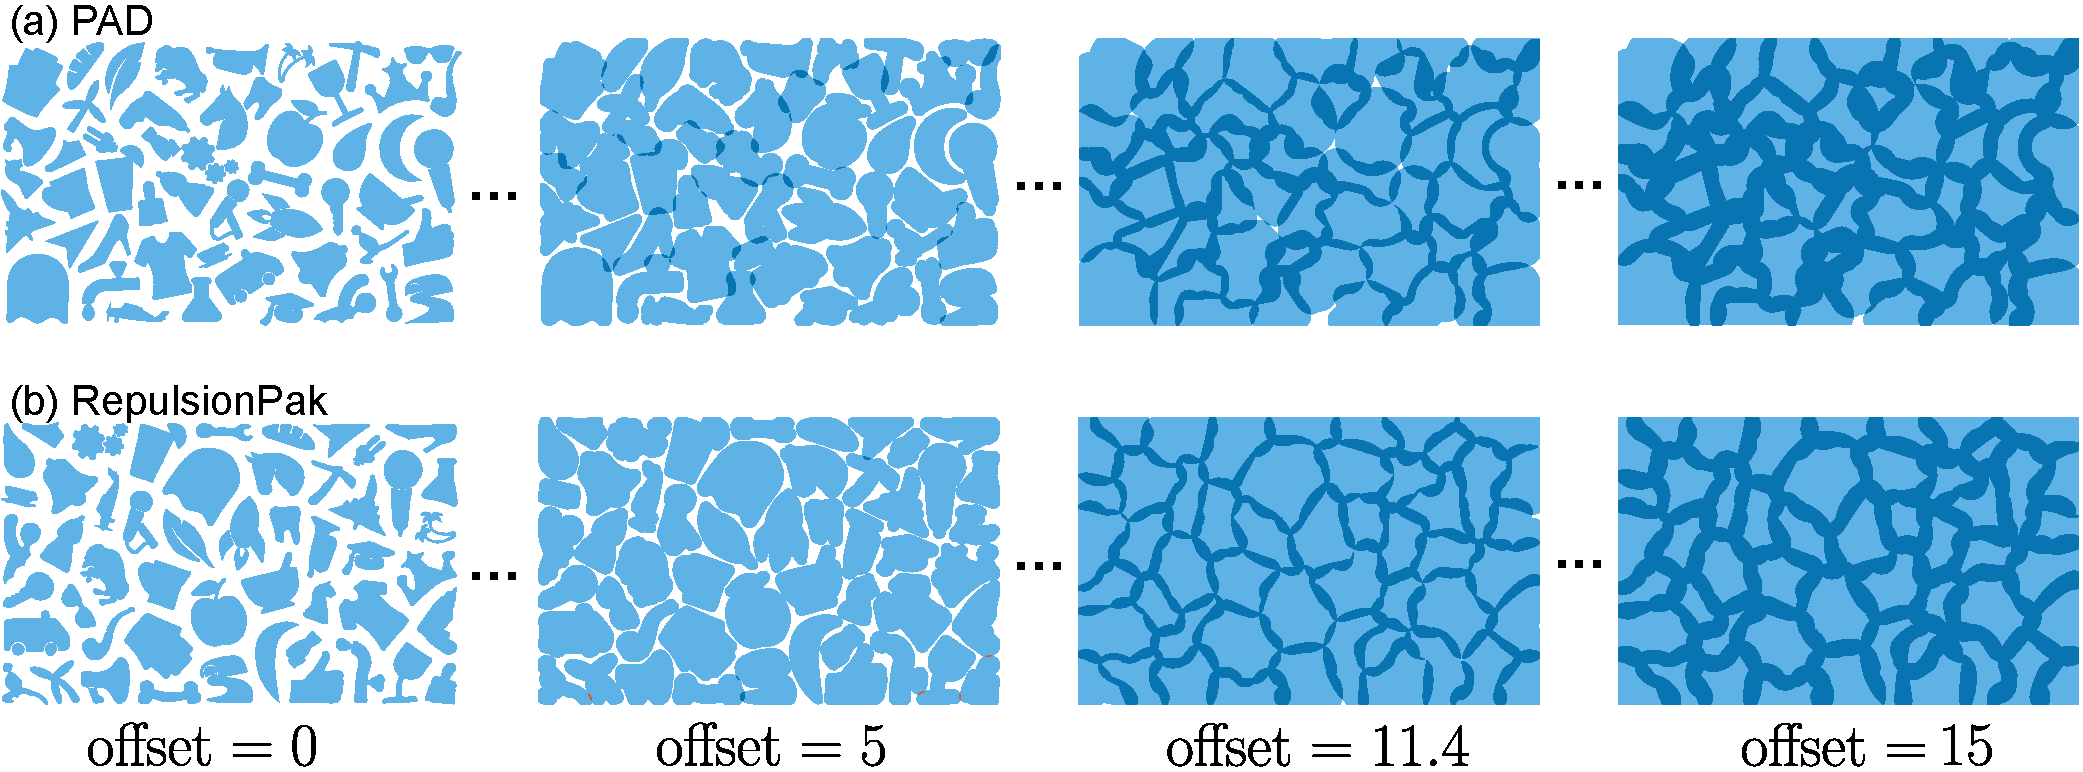
\includegraphics[width=1.0\textwidth]{figures/metrics/overlap_metric.pdf}
\caption[An illustration of offsetting elements outward]
{\label{fig_overlap_function}
    An illustration of offsetting elements outward. The packings have $d_\mathrm{gap} / 2 = 5.7$.  
    At an offset of 5, which is slightly less than $d_\mathrm{gap} / 2$,
    the overlap for the PAD packing is 1.462\% of the total area, while the overlap for our packing is only 0.039\%.
    At an offset of 11.4, which equals $d_\mathrm{gap}$, the PAD packing shows more empty space (1.05\%) than RepulsionPak (0.07\%).
    As the offset is increased, overlaps in the PAD packing create channels
  with uneven widths, whereas ours are more uniform.
  }
\end{figure}

\begin{figure}
\centering
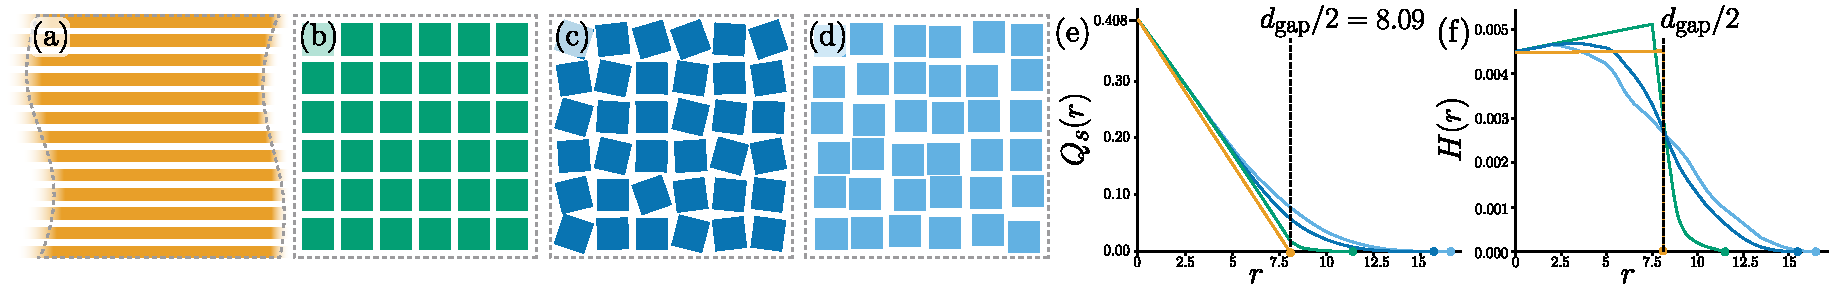
\includegraphics[width=1.0\textwidth]{figures/metrics/hsr_viz.pdf}
\caption[Spherical contact probabilities and distance histograms \newline for reference packings]
{\label{hsr_viz}
Spherical contact probabilities and distance histograms for 
reference packings.
A ``perfect packing'' of infinite stripes is shown in~(a),
followed by a square packing with the same area fraction and $d_\mathrm{gap}$
in~(b).  The square packing is then perturbed with random rotations in~(c)
and translations in~(d). The corresponding SCP functions and histograms are plotted
in~(e) and~(f).}
\end{figure}

\begin{figure}
\centering
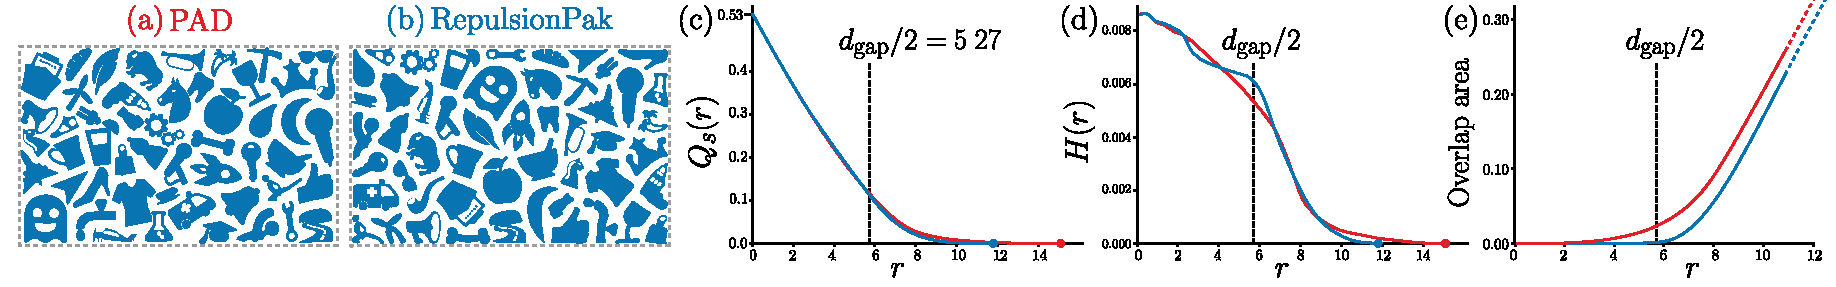
\includegraphics[width=1.0\textwidth]{figures/metrics/pad_comparison.pdf}
\caption[A comparison between a PAD~packing and a RepulsionPak packing \newline  with their corresponding SCPs]
{\label{pad_comparison}
    A comparison between a PAD~packing shown in~(a) and a RepulsionPak packing in~(b) 
    with their corresponding SCPs~(c), distance histograms~(d), and overlap functions~(e). 
  The PAD and RepulsionPak packings are calibrated
  to have the same negative space ratio.
    Our SCP is lower and shorter than the PAD's result,
    our histogram shows higher concentration around $d_\mathrm{gap} / 2$,
    indicating more even negative space,
    and our packing has a lower overlap function.
}
\end{figure}

\begin{figure}
\centering
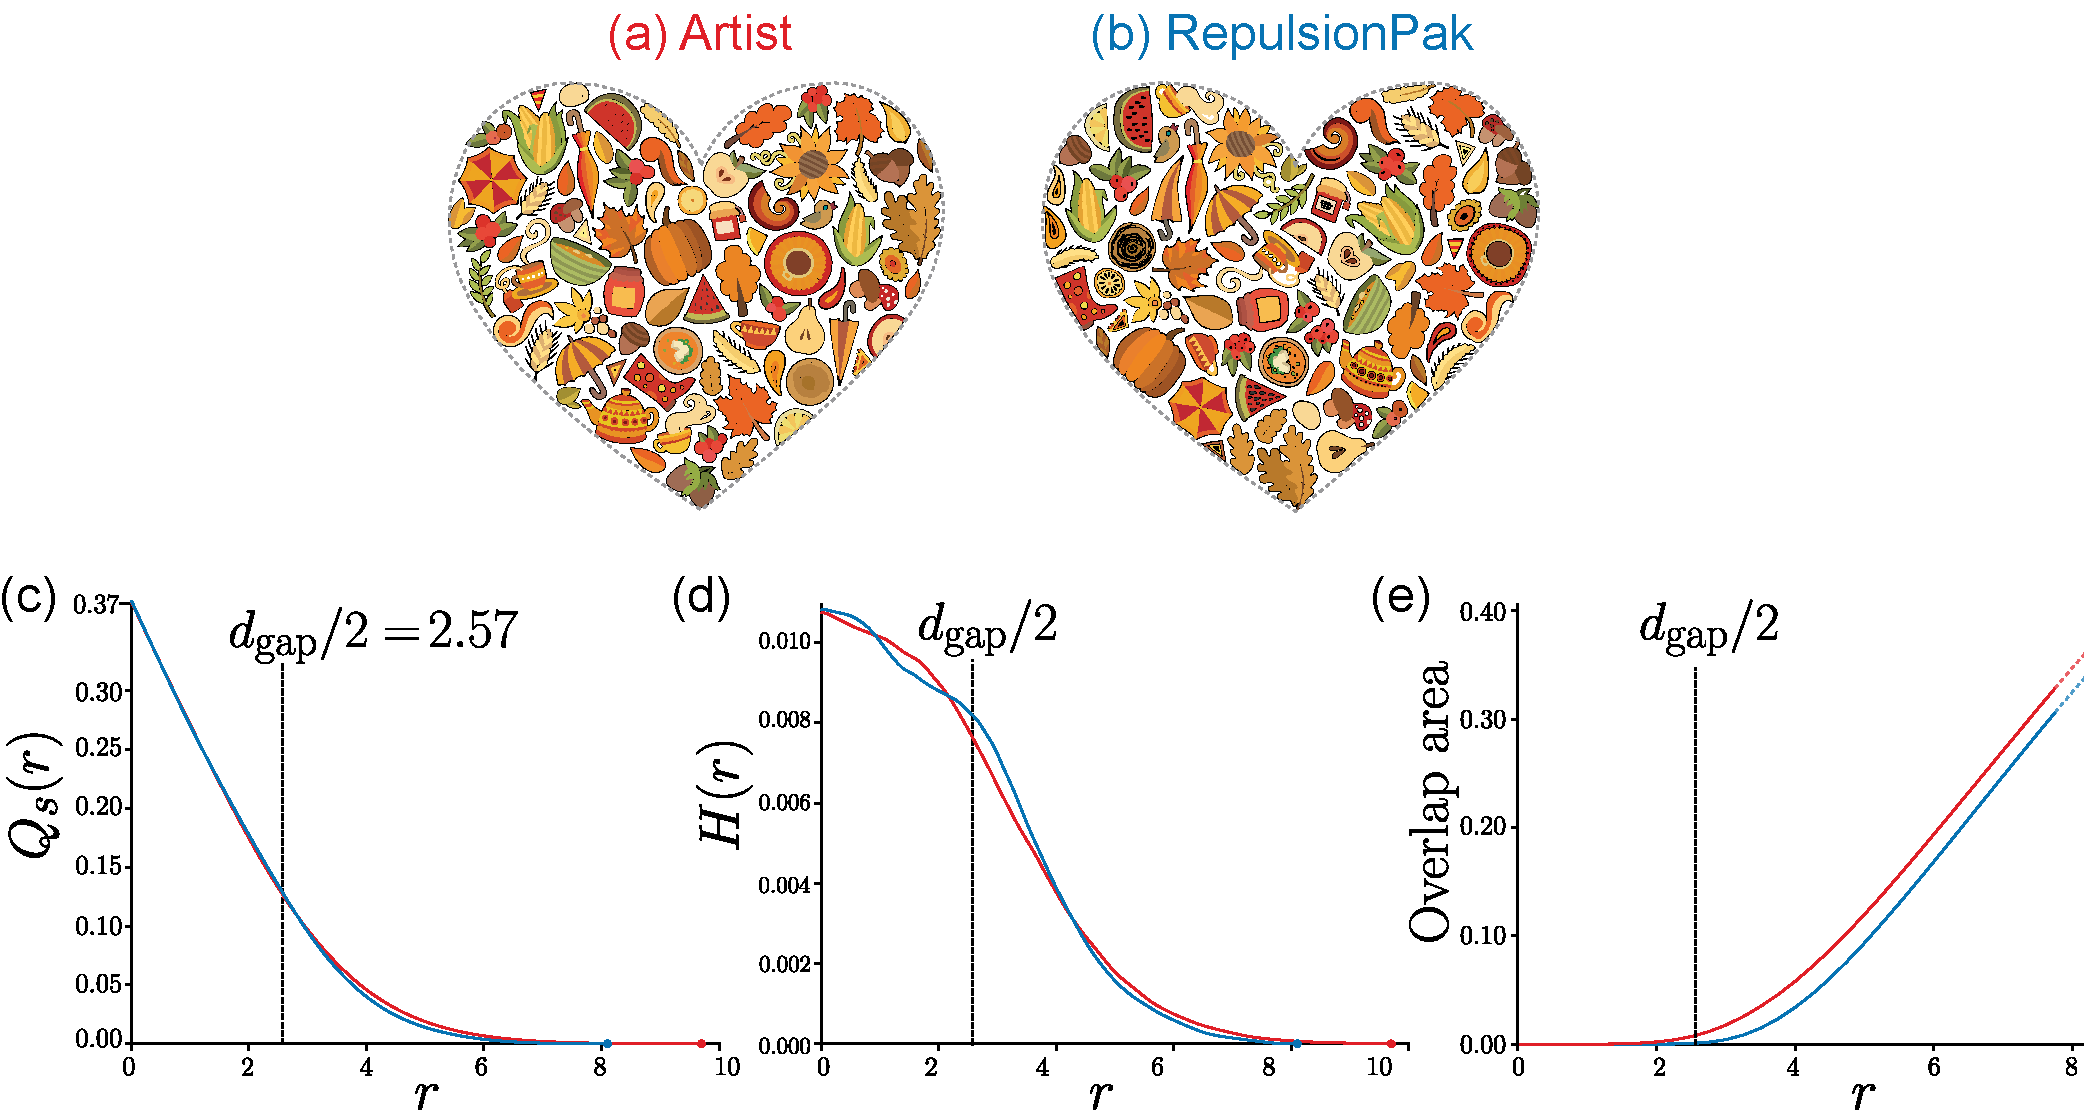
\includegraphics[width=1.0\textwidth]{figures/metrics/balabolka_comparison.pdf}
\caption[A comparison between the artist-made packing \newline  and a RepulsionPak packing]
{ \label{balabolka_comparison} 
    A comparison between the artist-made packing (Artist: Balabolka on Shutterstock) shown in~(a), and a RepulsionPak packing
  with the same elements in~(b).  We plot the corresponding SCPs~(c),
  distance histograms~(d), and overlap functions~(e).
    For comparison purposes we remove secondary elements from the artist's
  packing.  Our SCP is lower and shorter than the artist's result,
    our histogram shows more concentration around $d_\mathrm{gap} / 2$,
    and RepulsionPak also has a lower overlap function.
}
\end{figure}

\begin{figure}
\centering
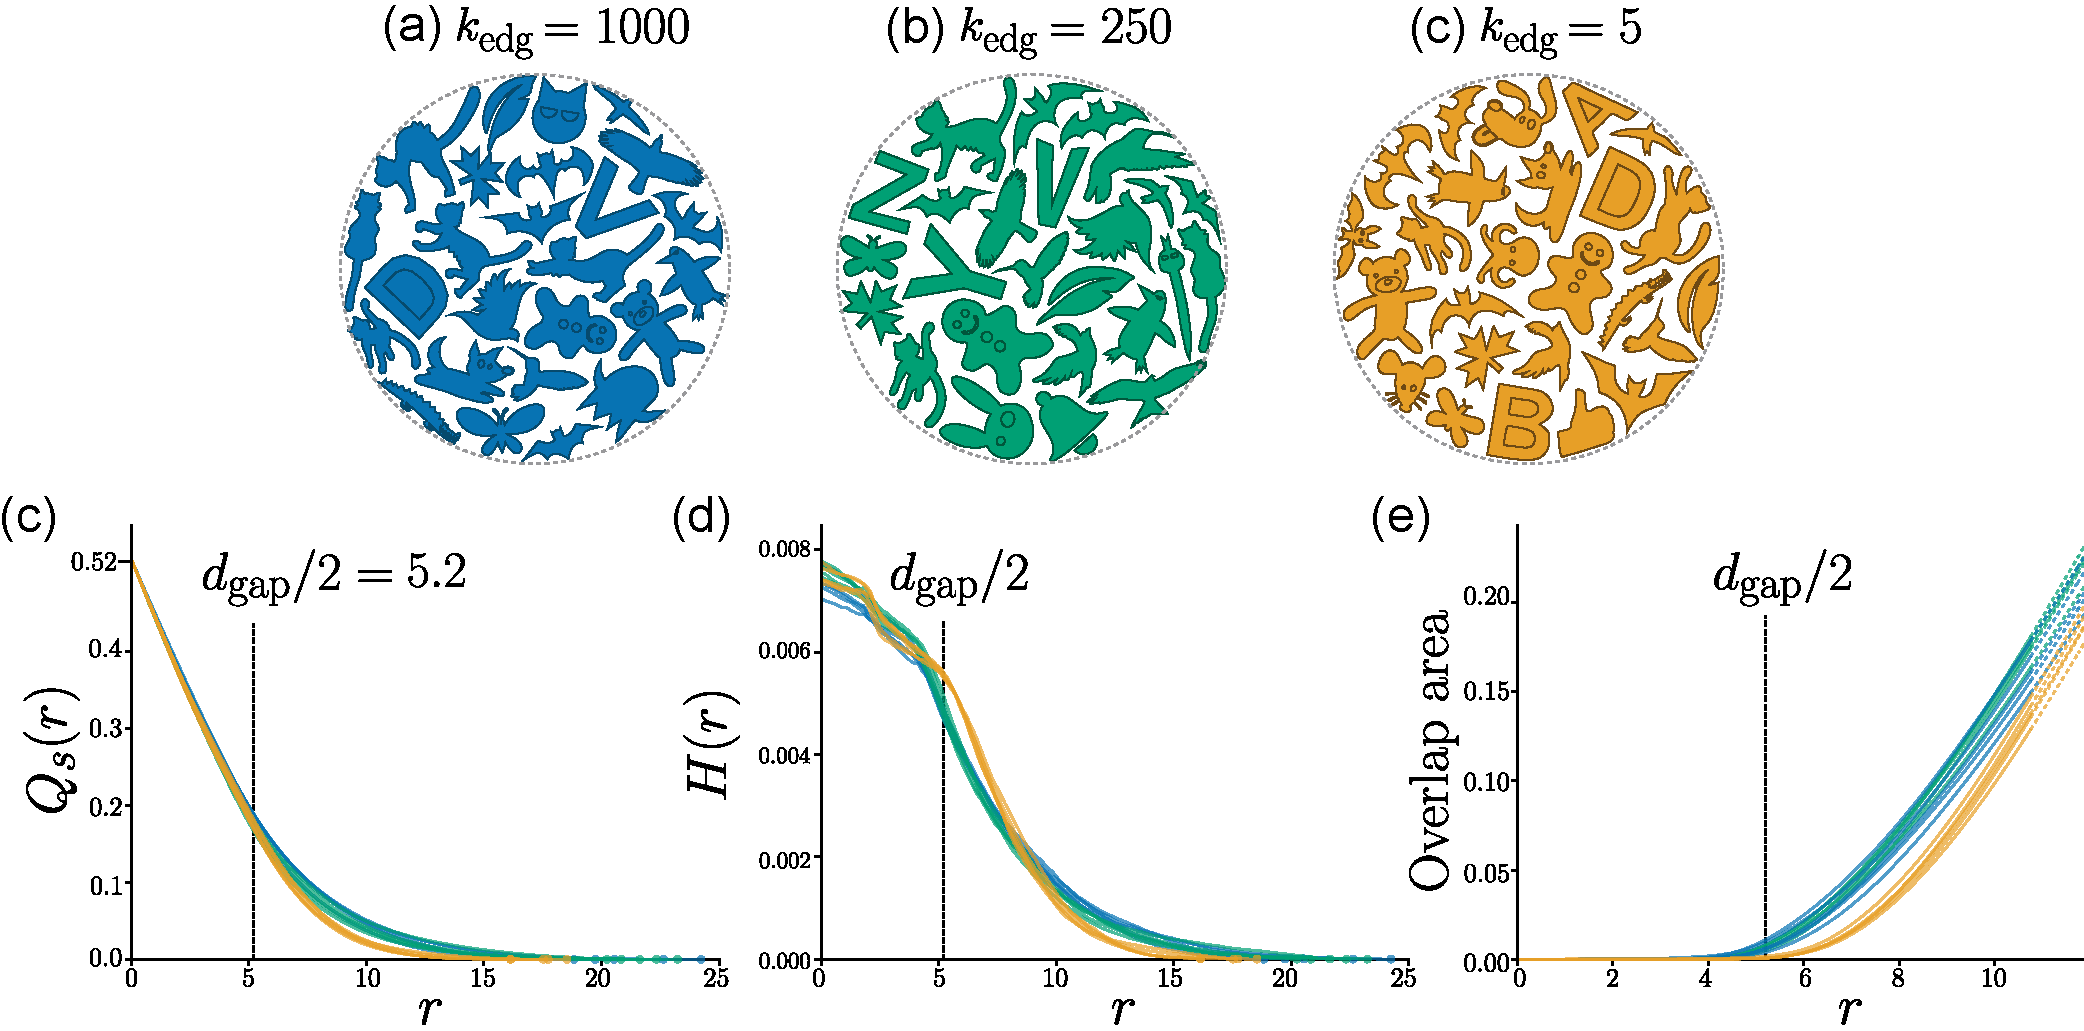
\includegraphics[width=1.0\textwidth]{figures/metrics/evaluation.pdf}
\caption[A demonstration of the effect of deformation \newline on the evenness of negative space]
{\label{fifteen_packings}
    A demonstration of the effect of deformation on the evenness of negative space.  
    The packings in (a), (b) and (c) are representative results using three values of the edge force strength $k_e$,
    from 
	rigid ($k_e=1000$) to moderate ($k_e=250$) to deformable ($k_e=5$).
% 	deformable ($k_e=5$) to moderate ($k_e=250$) to rigid ($k_e=1000$).
	We construct
    five random packings for each value of $k_e$, and plot their SCPs~(d), histograms~(e), and overlap functions~(f).
    Packings with the most deformation have steeper and shorter SCPs, 
    more histogram concentrations around $d_\mathrm{gap} / 2$, and lower overlap functions.
}
\end{figure}

\textbf{Comparison to PAD:} 
\newtext{
Figure~\ref{pad_comparison} compares
RepulsionPak and PAD~\cite{Kwan2016}.  Packing (a) is
a result from the PAD\ paper; Packing (b) was created with RepulsionPak using
the same elements, and calibrated to have the same negative space as~(a).
Note that the PAD\ packing actually has several overlapping elements
(for example, the tooth and the horse), but white haloes around
elements artfully conceal overlaps with little degradation in
visual quality.  Our packing avoids overlaps by design.
The SCP plot in~(c) shows that our packing has a lower value at $d_\mathrm{gap}/2$,
indicating more even negative space, and has a shorter tail,
indicating fewer large empty areas.
Our result also has a histogram bump around $d_\mathrm{gap}/2$, and 
a lower overlap function.
}

\textbf{Comparison to an artist-made packing:} 
\newtext{
In Figure~\ref{balabolka_comparison} we show a RepulsionPak result created 
using the elements from the artist-made packing.
Our packing was calibrated to match the artist's.
Looking closely, the artist's packing has a few elements 
separated by narrow gaps, such as the cherries and the corn on the top left.
Our result has fewer large empty gaps, as indicated by a short tail
in its SCP.
Our result also has a histogram bump around $d_\mathrm{gap}/2$, and a lower overlap function.
The result shows the effectiveness of the repulsion forces in successfully
discovering compatibilities in the element boundaries and filling the space effectively.
}

\textbf{Comparison to rigid packings}: 
\newtext{
To evaluate the
effect of deformation on negative space, we compute all three metrics under
increasing values of $k_e$, the edge spring strength.  Increasing $k_e$
allows the element meshes to resist deformation, ultimately
approximating a rigid packing algorithm.  We created 15 packings,
five for each of three values of $k_e$ (5, 250, and 1000).  Each packing
used 25 elements chosen at random from a library of 60, with
no secondary elements.  
All packings are partly calibrated: they all have the same negative
space ratio, but elements are chosen at random and have some
variation in their sizes.
As shown in Figure~\ref{fifteen_packings}, a low value of
$k_e$ leads to greater deformation and steeper SCPs.
The more pronounced histogram bump at $r=d_\mathrm{gap}/2$ suggests
more even negative space.
The lower overlap functions indicate fewer narrow gaps between elements.
}

%%%%%%%%%%%%%%%%%%%%%%%%%%%%%%%%%%%%%%%%%%%%%%%%%%%%%%%%%%
\section{Conclusions and Future Work}
%%%%%%%%%%%%%%%%%%%%%%%%%%%%%%%%%%%%%%%%%%%%%%%%%%%%%%%%%%

\newtext{
We hypothesized that the evenness of negative space is an indicator
for the quality of a packing. 
Negative space between elements should be uniform in width.
we validate our deformation-driven approach using overlap functions,
spherical contact probability functions, and distance histograms.
}

\begin{itemize}

\item We would like to conduct experiments that investigate the
  extent to which quantitative measurements of the evenness of negative
  space in a packing correlate with the human perception of a
  packing's quality.  In informal evaluations, some viewers found that
  the packing in Figure~\ref{balabolka_comparison}b, created with RepulsionPak,
  was packed more tightly than the artist's packing in
  Figure~\ref{balabolka_comparison}a, even though both have the same total
  amount of negative space.

\item Our validation metrics are all based on Minkowski sums or
  differences with discs, corresponding to a form of shape offsetting
  where corners become round.  The result of this rounding is visible in
  our graphs, for example in the gradual flattening of the SCP for
  the squares in Figure~\ref{hsr_viz}e.  It would be worthwhile to repeat
  these measurements using mitered offsetting, and to evaluate whether
  rounded or mitered offsetting is a closer match to human perceptual
  judgment of evenness.

\item When comparing calibrated packings, SCPs communicate 
  differences in the evenness of negative space, but the differences 
  between SCPs can be subtle.  In addition to distance histograms, 
  we would like to investigate other visualizations of this information
  that might amplify these differences to make evaluation easier.

\item We would like to develop additional metrics to evaluate
  how well an ornamental design fulfills other design principles.
  A measure of element deformation in a composition would permit 
  a comparison against future deformation-driven techniques.
  \newtext{In Chapter~\ref{chapter_flowpak}, we argue that visual flow and
  ``uniformity amidst variety'' are important to attractive packings.} 
  In another study, Wong et al.~\cite{Wong1998} describe basic design
  principles for decorative arts: repetition, balance, and conformation
  to geometric constraints.  The rigorous expression of aesthetic principles
  is a fascinating area for future research.

\item \newtext{All three metrics are only for evaluating 2D packings.
  While they extend naturally to three purely spatial
  dimensions, it is not clear whether they can be 
  adapted to the spacetime context.  
  We would like to investigate
  spatial statistics for the quality of animated packings that correlate
  with human perceptual judgments.}

\end{itemize}
